\documentclass[11pt]{article}
\usepackage[a4paper,landscape,margin=0.72in]{geometry}
\usepackage[T1]{fontenc}
\usepackage{lmodern}
\usepackage{amsmath}
\usepackage{amssymb}
\usepackage{graphicx}
\usepackage{hyperref}
\title{A sufficient condition for the actual quintic coordinate ring to be a domain}
\author{Formal proof packet}
\date{28 October 2026}
\begin{document}
\maketitle
\noindent This report records an explicitly conditional theorem. It adds no target result, experiment, or cost ratio. The editable SVG, CSV gate table, Lean source, and compiler log accompany this PDF.

\section*{Checked boundary}
Let $K$ be any field and $f=x^5+a_3x^3+a_2x^2+a_1x+a_0$. Suppose there are polynomials $t,u\in K[x]$ with $f=tu$, $t$ prime, and $t\nmid u$. The checked Eisenstein lemma gives irreducibility of $Y^2-f(X)$ over $K[X][Y]$. The new Lean theorems then establish that $K[x,y]/(y^2-f(x))$ is a domain, its localization at any rational curve point is a domain, and the corresponding actual weighted-$\operatorname{Proj}$ stalk is a domain.

The factor witness is a visible hypothesis. The current Lean packet does \emph{not} derive it from separability or odd degree. The proof does not require a characteristic assumption once the witness is supplied. The source formalizes no local DVR, divisor, $\mathrm{Pic}^0$ identity, compiled-law semantics, or cost claim.

\section*{Verification and next gates}
The direct Lean 4.34.1 compile exited zero using Mathlib revision
\par\noindent\texttt{d13f23b723b8a846827a245b89c10fc7d3f11612}.
The four printed theorem audits list only \texttt{propext}, \texttt{Classical.choice}, and \texttt{Quot.sound}; no \texttt{sorryAx}. Lean source SHA-256 is
\par\noindent{\small\texttt{4ead48655a0379aaac0107324236231aa122b32ed1efb1911409865a455d05da}}.

The next formal implication is: separability gives squarefreeness, a nonconstant quintic has an irreducible factor, and squarefreeness prevents its square from dividing $f$. The first implication is available as \texttt{Separable.squarefree} in pinned Mathlib; extraction and transport of the factor witness into the one-variable MvPolynomial representation remain to be compiled. The local maximal ideal must then be shown principal to infer a DVR. The exact statuses are in \texttt{affine-prime-factor-domain.csv}.

\clearpage
\section*{Proof dependencies and open gates}
\begin{center}
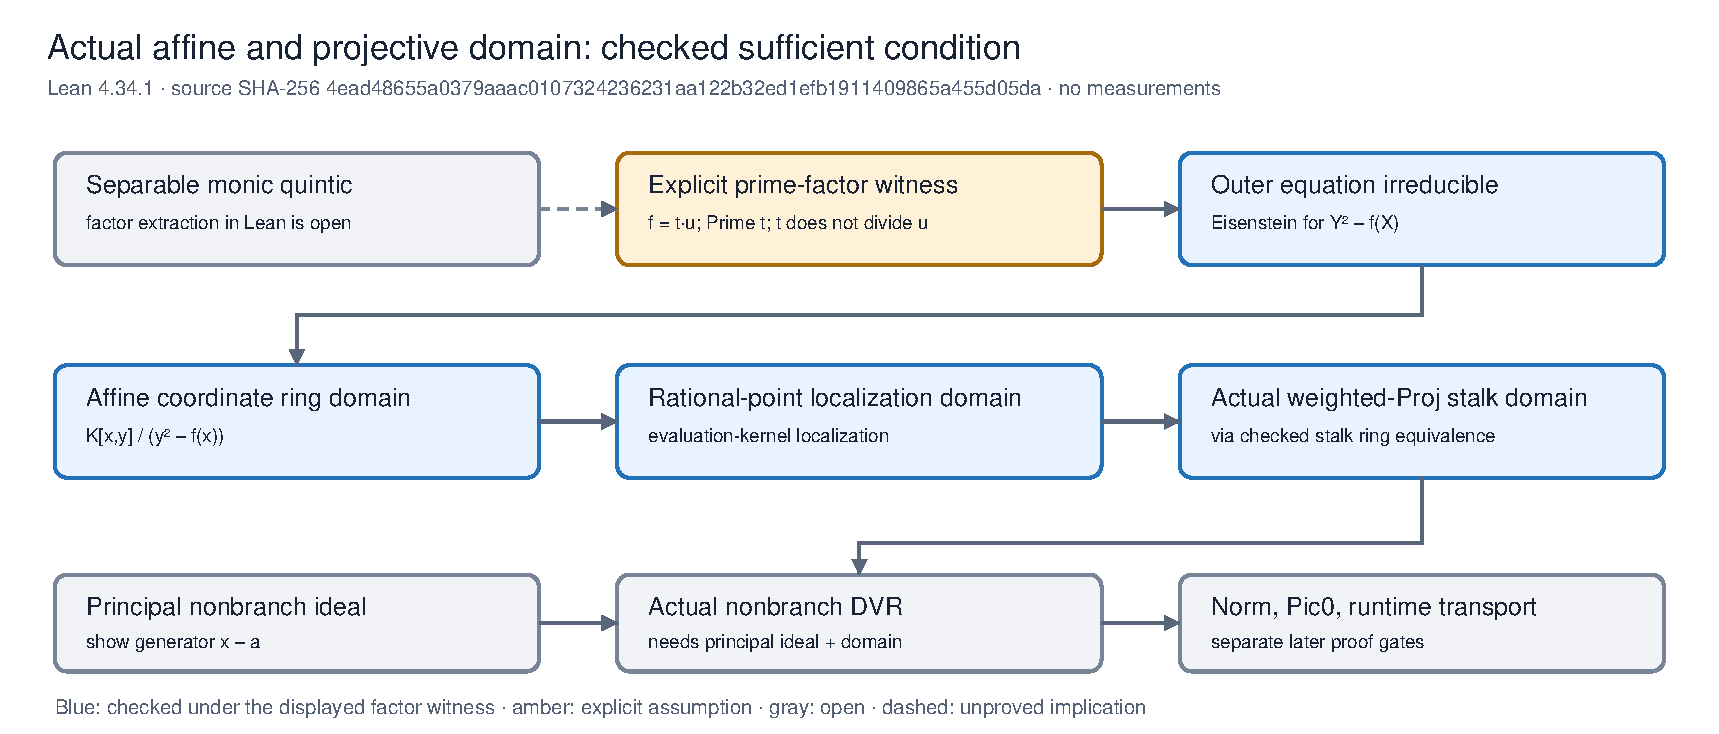
\includegraphics[width=0.96\textwidth,height=0.76\textheight,keepaspectratio]{affine-prime-factor-domain-figure.pdf}
\end{center}
\noindent Blue nodes are checked under the displayed factor witness. Amber is that explicit assumption. Gray nodes and the dashed implication are open. Arrows are proof dependencies, not performance measurements.
\end{document}
